\section{Auswertung}
\label{sec:Auswertung}

\subsection{Kennlinien der Hochvakuumdiode}
\label{sec:a}
Die für die Anodenspannung und den Anodenstrom aufgenommenen Werte
bei den Heizstömen von $I_\text{H} = \num{2}$ bis $\SI{2.4}{\ampere}$
sind in den Tabellen \ref{taba} bis \ref{tabe} zu sehen.

\begin{table}\caption{Die Länge der Zylinder und die Spannung mit den jeweiligen Zeitenpunkten der Ausschläge.}
\label{taba}
\centering
\sisetup{round-mode = places, round-precision=2, round-integer-to-decimal=true}
\begin{tabular}{S[]S[]S[]S[]S[]} 
\toprule
{$l/ \si{\milli\meter}$} & {$U_1/ \si{\volt}$} & {$t_1/ \si{\micro\second}$} & {$U_2/ \si{\volt}$} & {$t_2/ \si{\micro\second}$}\\
\midrule
120.8 & 1.29 & 0.6 & 0.17 & 88.7\\
102.3 & 1.27 & 0.5 & 0.2 & 76.5\\
80.5 & 1.33 & 0.6 & 0.76 & 59.8\\
40.4 & 1.33 & 0.5 & 1.34 & 30.2\\
31.1 & 1.29 & 0.5 & 1.37 & 23.8\\
\bottomrule
\end{tabular}\end{table}
\begin{table}\caption{Die angelegte Spannung des elektrischen Feldes innerhalb des Geiger-Müller-Zählrohrs, die Anzahl der jeweils gemessenen Impulse und der Strom innerhalb des Geiger-Müller-Zählrohrs.}
\label{tabb}
\centering
\sisetup{round-mode = places, round-precision=2, round-integer-to-decimal=true}
\begin{tabular}{c c S[]} 
\toprule
{$U / \si{\volt}$} & {$\frac{N}{\SI{130}{\second}}$} & {$I / \si{\ampere}$}\\
\midrule
320 & 11298 & 0.1\\
400 & 11820 & 0.2\\
480 & 12135 & 0.3\\
540 & 12301 & 0.35\\
560 & 12068 & 0.4\\
600 & 12354 & 0.45\\
640 & 12403 & 0.5\\
660 & 12507 & 0.55\\
680 & 12659 & 0.6\\
\bottomrule
\end{tabular}\end{table}
\begin{table}\caption{Der Anodenstrom und der Kathodenstrom bei einer Beschleunigungsspannung von $U_\text{B} = \SI{25}{\kilo\volt}$ und einer Kathodenspannung $U_\text{K,1} = \SI{500}{\volt}$ und einer Kathodenspannung $U_\text{K,2} = \SI{300}{\volt}$ bei einem Blendenradius von $r_\text{B} = \SI{5}{\milli\meter}$.}
\label{tabc}
\centering
\sisetup{round-mode = places, round-precision=2, round-integer-to-decimal=true}
\begin{tabular}{S[]S[]S[]} 
\toprule
{$I_\text{K} / \si{\milli\ampere}$} & {$I_\text{K,1} / \si{\nano\ampere}$} & {$I_\text{K,2} / \si{\nano\ampere}$}\\
\midrule
1.0 & 2.6 & 2.4\\
0.95 & 2.5 & 2.4\\
0.9 & 2.4 & 2.2\\
0.85 & 2.3 & 2.1\\
0.8 & 2.2 & 2.0\\
0.75 & 2.1 & 1.9\\
0.7 & 1.9 & 1.8\\
0.65 & 1.8 & 1.6\\
0.6 & 1.6 & 1.5\\
0.55 & 1.5 & 1.4\\
0.5 & 1.4 & 1.3\\
0.45 & 1.2 & 1.2\\
0.4 & 1.1 & 1.0\\
0.35 & 0.9 & 0.9\\
0.3 & 0.8 & 0.8\\
0.25 & 0.6 & 0.6\\
0.2 & 0.5 & 0.5\\
0.15 & 0.4 & 0.4\\
0.1 & 0.1 & 0.2\\
0.05 & 0.1 & 0.1\\
\bottomrule
\end{tabular}\end{table}
\begin{table}\caption{Laufzeiten und Spannungen der reflektierten Impulse bei dem Modell des Auges.}
\label{tabd}
\centering
\sisetup{round-mode = places, round-precision=2, round-integer-to-decimal=true}
\begin{tabular}{S[]S[]} 
\toprule
{$t_1/ \si{\micro\second}$} & {$U_1/ \si{\volt}$}\\
\midrule
1.0 & 1.38\\
11.7 & 1.0\\
16.1 & 1.25\\
22.9 & 0.95\\
72.2 & 0.4\\
\bottomrule
\end{tabular}\end{table}
\begin{table}\caption{Die Frequenz gegen den doppelten Wert der Amplitude der Brückenspannung.}
\label{tabe}
\centering
\sisetup{round-mode = places, round-precision=3, round-integer-to-decimal=true}
\begin{tabular}{S[]S[]} 
\toprule
{$f/\si{\Hz}$} & {$2 U_{Br}/\si{\V}$}\\
\midrule
20.0 & 1.68\\
50.0 & 1.62\\
100.0 & 1.32\\
150.0 & 0.952\\
200.0 & 0.664\\
250.0 & 0.404\\
300.0 & 0.248\\
400.0 & 0.0608\\
500.0 & 0.304\\
600.0 & 0.492\\
700.0 & 0.636\\
800.0 & 0.8\\
900.0 & 0.896\\
1000.0 & 0.96\\
1100.0 & 1.01\\
1200.0 & 1.04\\
1300.0 & 1.09\\
1400.0 & 1.13\\
1500.0 & 1.2\\
1600.0 & 1.19\\
1700.0 & 1.19\\
1800.0 & 1.22\\
1900.0 & 1.23\\
2000.0 & 1.28\\
2500.0 & 1.31\\
3000.0 & 1.37\\
4000.0 & 1.42\\
5000.0 & 1.41\\
6000.0 & 1.46\\
7000.0 & 1.41\\
10000.0 & 1.38\\
11000.0 & 1.35\\
12000.0 & 1.37\\
13000.0 & 1.34\\
14000.0 & 1.27\\
15000.0 & 1.31\\
16000.0 & 1.28\\
17000.0 & 1.31\\
18000.0 & 1.35\\
19000.0 & 1.35\\
20000.0 & 1.35\\
21000.0 & 1.35\\
22000.0 & 1.35\\
30000.0 & 1.35\\
\bottomrule
\end{tabular}\end{table}

\noindent Die Ströme sind in Abb. \ref{fig:plot1} jeweils gegen die Spannungen
aufgetragen.
\begin{figure}
    \centering
    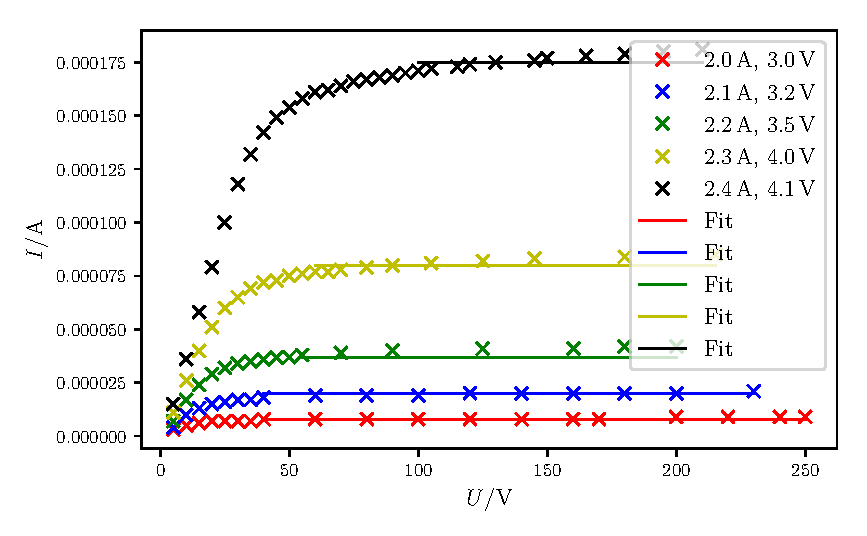
\includegraphics[width=15cm, height=9cm]{build/plot1.pdf}
    \caption{Die Anodenströme sind jeweils für die verschiedenen Heizströme/-Spannungen
    gegen die Anodenspannungen aufgetragen.}
    \label{fig:plot1}
\end{figure}

\noindent Aus der Abb. \ref{fig:plot1} lassen sich jeweils
die Sättigungsströme ablesen. Diese sind für die verschiedenen
Heizströme
\begin{align*}
    I_\text{H} = \SI{2.0}{\ampere} \Rightarrow I_\text{S} &= \SI{8e-6}{\ampere} \\
    I_\text{H} = \SI{2.1}{\ampere} \Rightarrow I_\text{S} &= \SI{20e-6}{\ampere} \\
    I_\text{H} = \SI{2.2}{\ampere} \Rightarrow I_\text{S} &= \SI{37e-6}{\ampere} \\
    I_\text{H} = \SI{2.3}{\ampere} \Rightarrow I_\text{S} &= \SI{80e-6}{\ampere} \\
    I_\text{H} = \SI{2.4}{\ampere} \Rightarrow I_\text{S} &= \SI{175e-6}{\ampere}.
\end{align*}

\subsection{Gültigkeitsbereich des Raumladungsgesetzes}
Der Exponent, der mittels einer linearen Regression
bestimmt wurde, ist
\begin{equation*}
    x = \num{1.18 \pm 0.03}.
\end{equation*}
%erwartet wird 1.5

\subsection{Anlaufstromgebiet der Diode und Bestimmung der Kathodentemperatur}
Die Werte für die Spannungen und Ströme im Anlaufstromgebiet
befinden sich in den Tabellen \ref{tabf} bis \ref{tabh}.

\begin{table}\caption{Die gemessene Gegenspannung und die dazu gehörende Stromstärke.}
\label{tabf}
\centering
\sisetup{round-mode = places, round-precision=1, round-integer-to-decimal=true}
\begin{tabular}{S[]S[]} 
\toprule
{$U / \si{\milli\volt}$} & {$I / \si{\nano\ampere}$}\\
\midrule
0.0 & 38.0\\
50.0 & 34.0\\
100.0 & 28.0\\
150.0 & 23.0\\
200.0 & 19.0\\
250.0 & 15.0\\
300.0 & 12.0\\
350.0 & 9.0\\
400.0 & 7.0\\
450.0 & 6.0\\
500.0 & 5.0\\
\bottomrule
\end{tabular}\end{table}
\begin{table}\caption{Die Gegenspannung und die dazu gehörende Stromstärke.}
\label{tabg}
\centering
\sisetup{round-mode = places, round-precision=1, round-integer-to-decimal=true}
\begin{tabular}{S[]S[]} 
\toprule
{$U / \si{\milli\volt}$} & {$I / \si{\nano\ampere}$}\\
\midrule
400.0 & 8.9\\
450.0 & 6.8\\
500.0 & 5.3\\
550.0 & 4.0\\
600.0 & 3.1\\
650.0 & 2.3\\
700.0 & 1.75\\
750.0 & 1.35\\
800.0 & 1.0\\
850.0 & 0.7\\
900.0 & 0.5\\
950.0 & 0.2\\
1000.0 & 0.1\\
\bottomrule
\end{tabular}\end{table}
\begin{table}\caption{Die gemessene Gegenspannung und die dazu gehörende Stromstärke.}
\label{tabh}
\centering
\sisetup{round-mode = places, round-precision=1, round-integer-to-decimal=true}
\begin{tabular}{S[]S[]} 
\toprule
{$U / \si{\milli\volt}$} & {$I / \si{\nano\ampere}$}\\
\midrule
850.0 & 0.69\\
900.0 & 0.52\\
950.0 & 0.37\\
1000.0 & 0.22\\
\bottomrule
\end{tabular}\end{table}

\noindent Die Temperatur im Anlaufstromgebiet ist %Gleichung?
\begin{equation*}
    T = \SI{2.44(12)e3}{\kelvin}.
\end{equation*}
%plot 
%Formel am ende von 6
%

\subsection{Leistungsbilanz des Heizstromkreises und Abschätzung der Kathodentemperatur}
Die in Teil \ref{sec:a} verwendeten Heizleistungen sind
\begin{align*}
    P_\text{1} &= \SI{6.00}{\watt} \\
    P_\text{2} &= \SI{6.72}{\watt} \\
    P_\text{3} &= \SI{7.7}{\watt} \\
    P_\text{4} &= \SI{9.20}{\watt} \\
    P_\text{5} &= \SI{9.84}{\watt}.
\end{align*}

\noindent Die Werte für die emittierende Kathodenoberfläche $f$ und den
Emissionsgrad der Oberfläche $\eta$ sind
\begin{align*}
    f &= \SI{0.32}{\centi\meter\squared} \\
    \eta &= \num{0.28}.
\end{align*}

\noindent Daraus ergeben sich mit der Gleichung \eqref{eqn:} 
die Temperaturen
\begin{align*}
    T_\text{1} &= \SI{1768.87}{\kelvin} \\
    T_\text{2} &= \SI{1829.38}{\kelvin} \\
    T_\text{3} &= \SI{1903.15}{\kelvin} \\
    T_\text{4} &= \SI{2001.74}{\kelvin} \\
    T_\text{5} &= \SI{2039.71}{\kelvin}.
\end{align*}
%Gleichung anleitung d

\subsection{Austrittsarbeit für Wolfram}
Die berechneten Austrittsarbeiten $e_0 \phi$ sind
\begin{align*}
    (e_0 \phi)_\text{1} &= \SI{9.93e-19}{\electronvolt} \\
    (e_0 \phi)_\text{2} &= \SI{1.01e-18}{\electronvolt} \\
    (e_0 \phi)_\text{3} &= \SI{1.03e-18}{\electronvolt} \\
    (e_0 \phi)_\text{4} &= \SI{1.07e-18}{\electronvolt} \\
    (e_0 \phi)_\text{5} &= \SI{1.07e-18}{\electronvolt}.
\end{align*}

\noindent Der sich daraus ergebende Mittelwert ist
\begin{equation*}
    (e_0 \phi)_\text{mittel} = \SI{100000000}{\electronvolt}.
\end{equation*}